\begin{figure*}
  \centering

\begin{minipage}{\textwidth}
\begin{subfigure}[b]{0.4\textwidth}
\centering
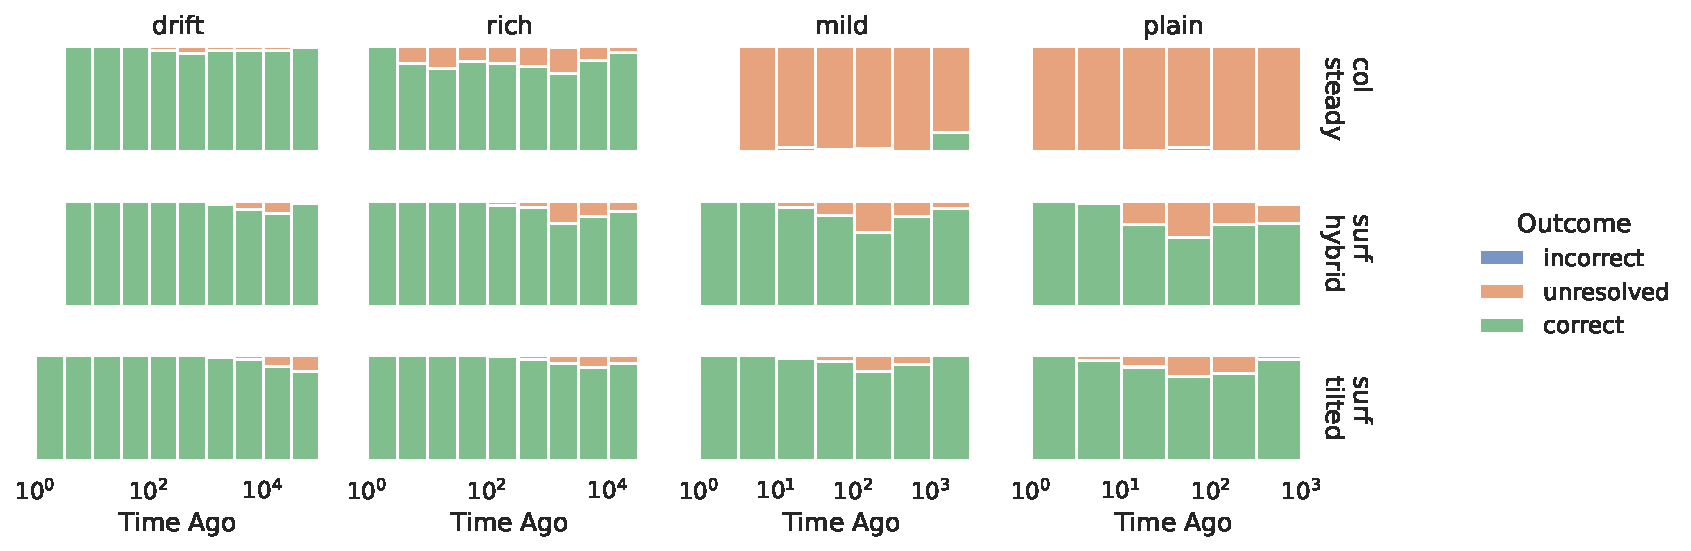
\includegraphics[height=1.2in,trim={0 0 5cm 0},clip]{binder/binder/teeplots/annotation-size-bits=256+col=scenario+differentia-width-bits=8+hue=outcome+kind=hist+multiple=fill+row=algo+scale=npop65536-ngen100000+viz=displot+x=time-ago+ext=}
\caption{256-bit annotation, byte differentia}
\end{subfigure}%
\begin{subfigure}[b]{0.6\textwidth}
\centering
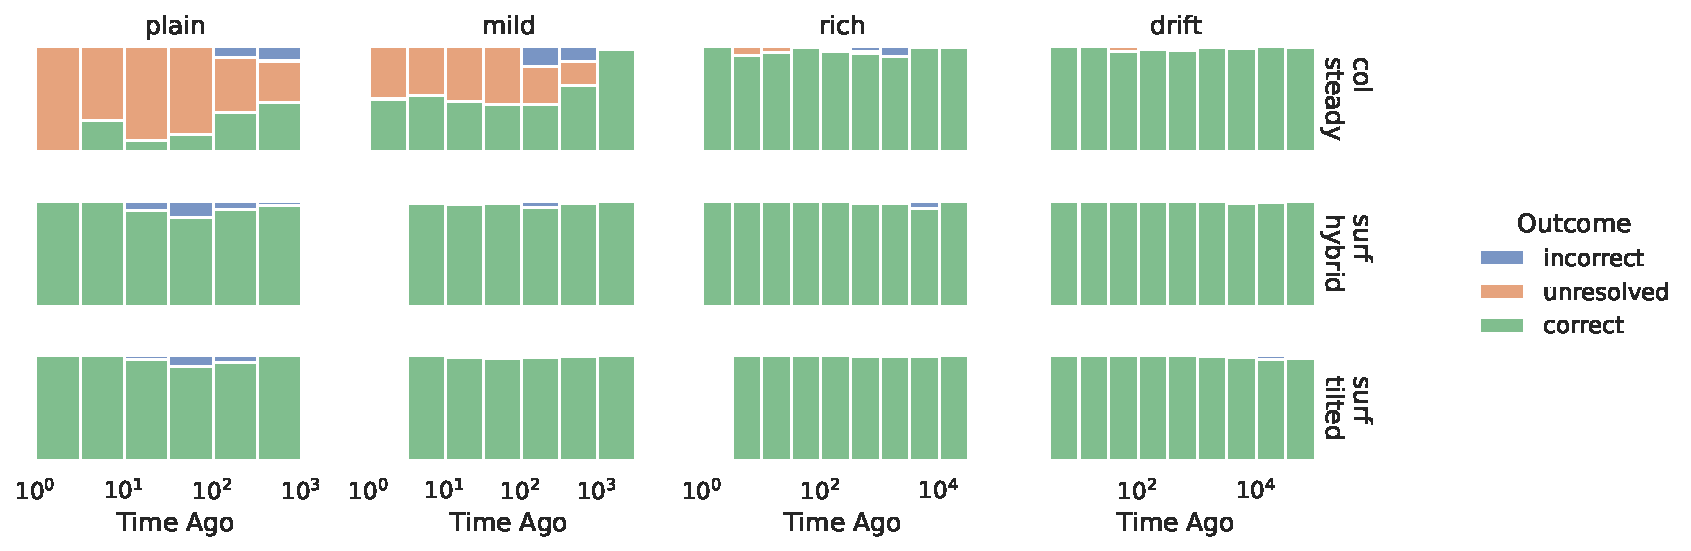
\includegraphics[height=1.2in]{binder/binder/teeplots/annotation-size-bits=256+col=scenario+differentia-width-bits=1+hue=outcome+kind=hist+multiple=fill+row=algo+scale=npop65536-ngen100000+viz=displot+x=time-ago+ext=}
\caption{256-bit annotation, bit differentia}
\end{subfigure}
% \begin{subfigure}[b]{0.6\textwidth}
% \centering
% 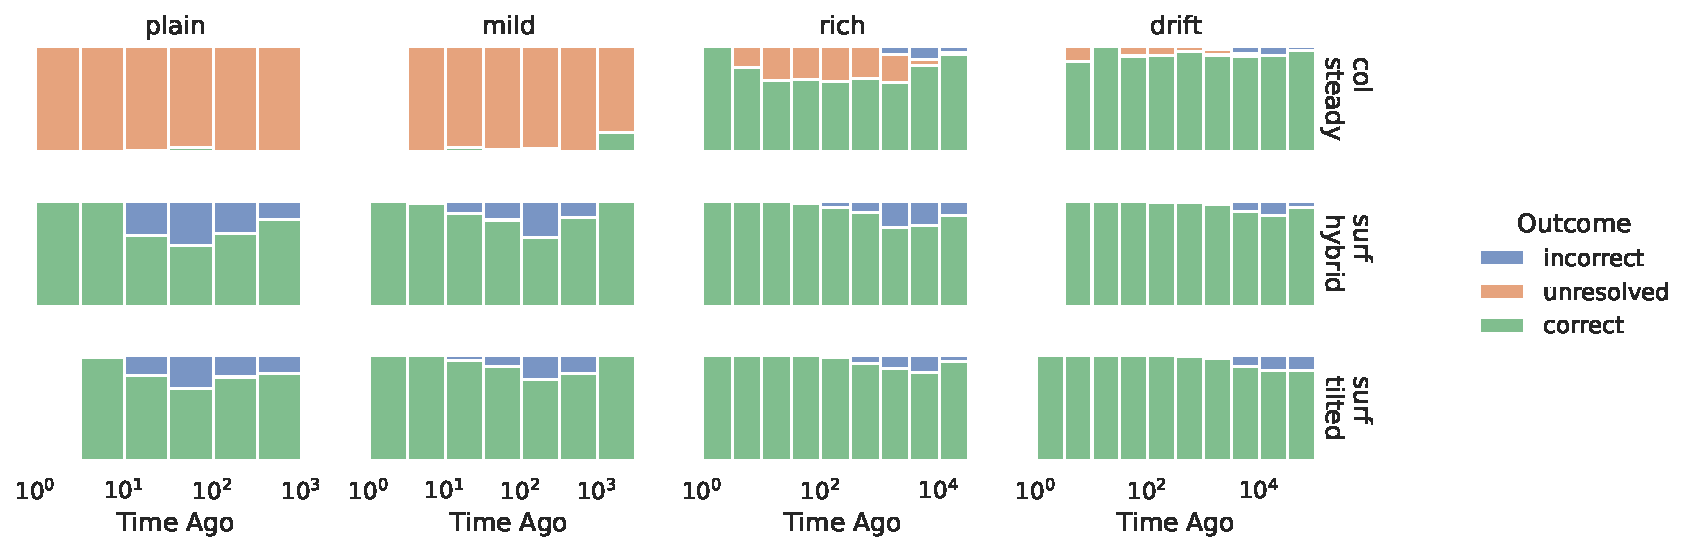
\includegraphics[height=1.2in]{binder/binder/teeplots/annotation-size-bits=32+col=scenario+differentia-width-bits=1+hue=outcome+kind=hist+multiple=fill+row=algo+scale=npop65536-ngen100000+viz=displot+x=time-ago+ext=}
% \caption{32-bit annotation, bit differentia}
% \end{subfigure}
\end{minipage}
% \begin{subfigure}[b]{0.4\textwidth}
%   \centering
%   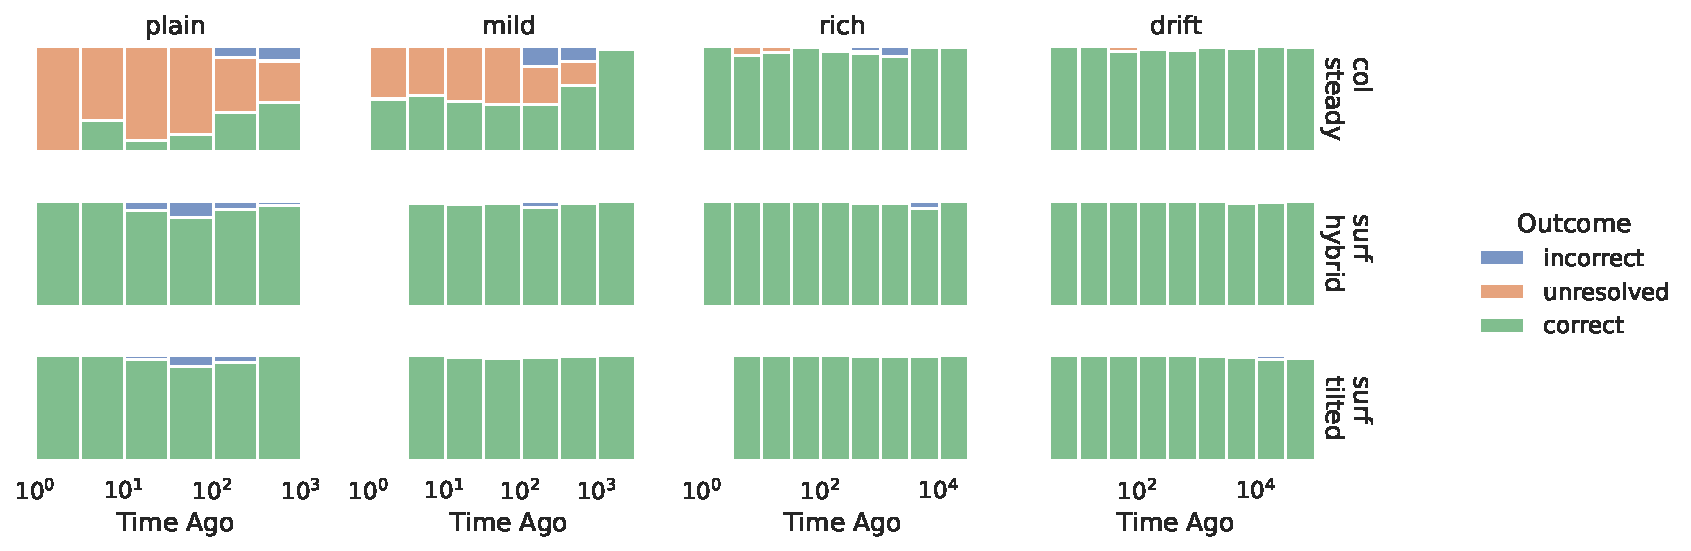
\includegraphics[height=1.2in,trim={0 0 5cm 0},clip]{binder/binder/teeplots/annotation-size-bits=256+col=scenario+differentia-width-bits=1+hue=outcome+kind=hist+multiple=fill+row=algo+scale=npop65536-ngen100000+viz=displot+x=time-ago+ext=}
%   \caption{reconstruction outcomes; 256-bit annotation, bit differentia}
%   \end{subfigure}%
  \begin{subfigure}[b]{\textwidth}
    \centering
    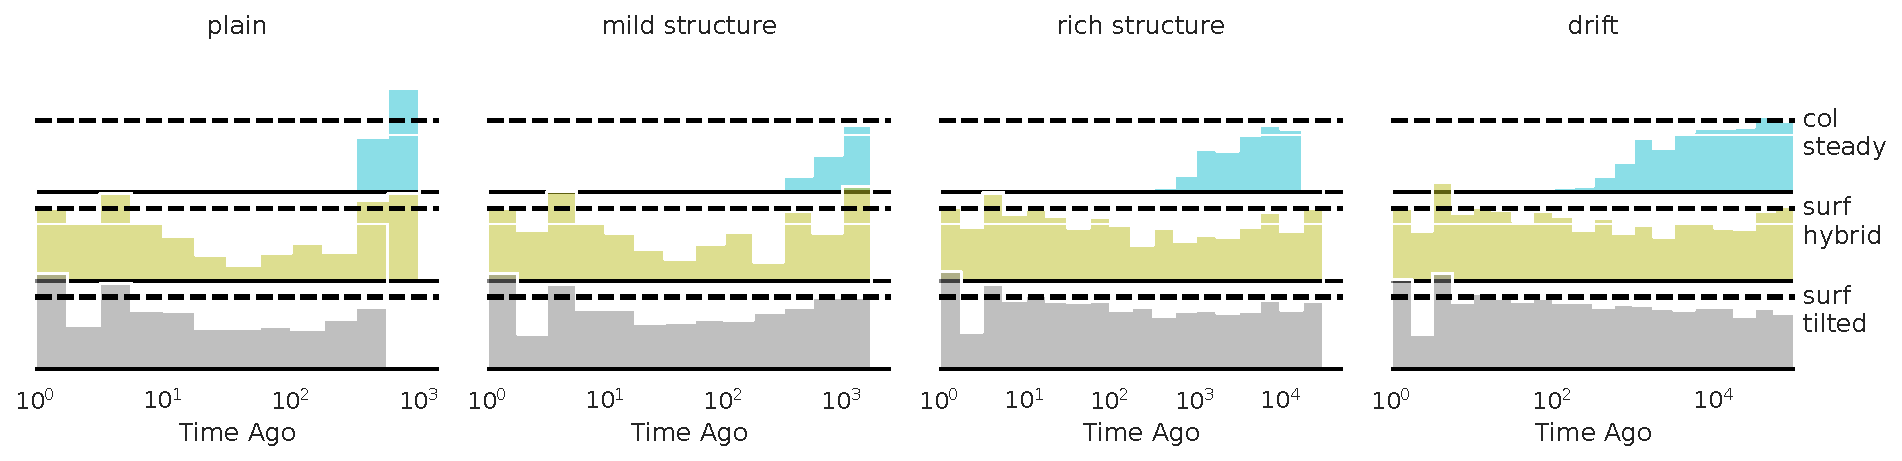
\includegraphics[width=0.8\linewidth]{binder/binder/teeplots/annotation-size-bits=256+col=scenario+differentia-width-bits=8+hue=kind+row=algo+scale=npop65536-ngen100000+viz=joyhist+x=time-ago+ext=}
    \caption{reconstruction node densities; 256-bit size, byte differentia}
  \end{subfigure}%
  \caption{%
  \textbf{How do reconstruction outcomes differ by retention policy and differentia size?}
  Top panels shows reconstruction outcome proportions for branching events, binned by time ago (ranging from most recent to most ancient).
  Bottom panel shows internal node count relative to reference trees (dashed line), also binned by time ago.
  Facet columns differentiate evolutionary regimes and facet rows correspond to steady, hybrid, and tilted retention policies.
  For hybrid and tilted policies under byte differentia, almost no phylogeny components are incorrectly reconstructed, but some components are unresolved.
  Under bit differentia, higher fractions of components are correctly resolved.
  However, unlike byte differentia, a small fraction of components are incorrectly reconstructed.
  Without strong factors maintaining phylogenetic richness (i.e., mild/plain structure conditions), large fractions of phylogeny components are unresolved under the steady policy.
  This can be attributed far below reference node counts for recent time, due to lack of retained recent differentia.
  Depressions in hybrid and tilted policy node counts can also be seen, corresponding to discussedunresolved phylogenetic components with byte differentia.
  }
  \label{fig:recency-structure}

\end{figure*}
